Hello



\begin{figure}[!ht]
\centering
\subfloat[Naive Bayes]{\includegraphics[width=.5\textwidth]{../images/nb_acc_vs_dim_pca_sr.png}}
\subfloat[SVM]{\includegraphics[width=.5\textwidth]{../images/svm_acc_vs_dim_pca_sr.png}}
\caption{Accuracy vs. dim. PCA Projection}
\label{fig:pca_acc_vs_proj_dim}
\end{figure}

In analysis, here, mention something about how with svm model complexity scales with number of training examples, not dimensionality of feature space. Also, point out that it makes sense to use linear kernel, rather than rbf, because of COD. 


\begin{center}
\begin{figure}[!ht]
\centering
\includegraphics[width=.5\textwidth]{../images/accuracy_vs_dim_randproj.png}
\caption{Naive Bayes Acc. vs. num dim Rand. Projection}
\label{fig:nb_rand_proj}
\end{figure}
\end{center}

%also include naive bayes small pca vs. naive bayes pca. If it was just an issue of underfit gaussians, nonsmall would do better for bigger training sets, but it doesn't. 


\begin{figure}[!ht]
\centering
\subfloat[Reduced Data Sparsity]{\includegraphics[width=.5\textwidth]{../images/PCAsparsityDensity.png}}
\subfloat[Cumulative Covariance]{\includegraphics[width=.5\textwidth]{../images/pca_cumsum.png}}
\caption{Characteristics of PCA-reduced data}
\label{fig:PCA_RED}
\end{figure}



\begin{center}
\begin{figure}[!ht]
\centering
\includegraphics[width=.5\textwidth]{../images/nb_5_vs_50.png}
\caption{Naive Bayes Accuracy vs. Train set size for 5 and 50 PCA dims.}
\label{fig:5_vs_50_pca}
\end{figure}
\end{center}

\begin{center}
\begin{figure}[!ht]
\centering
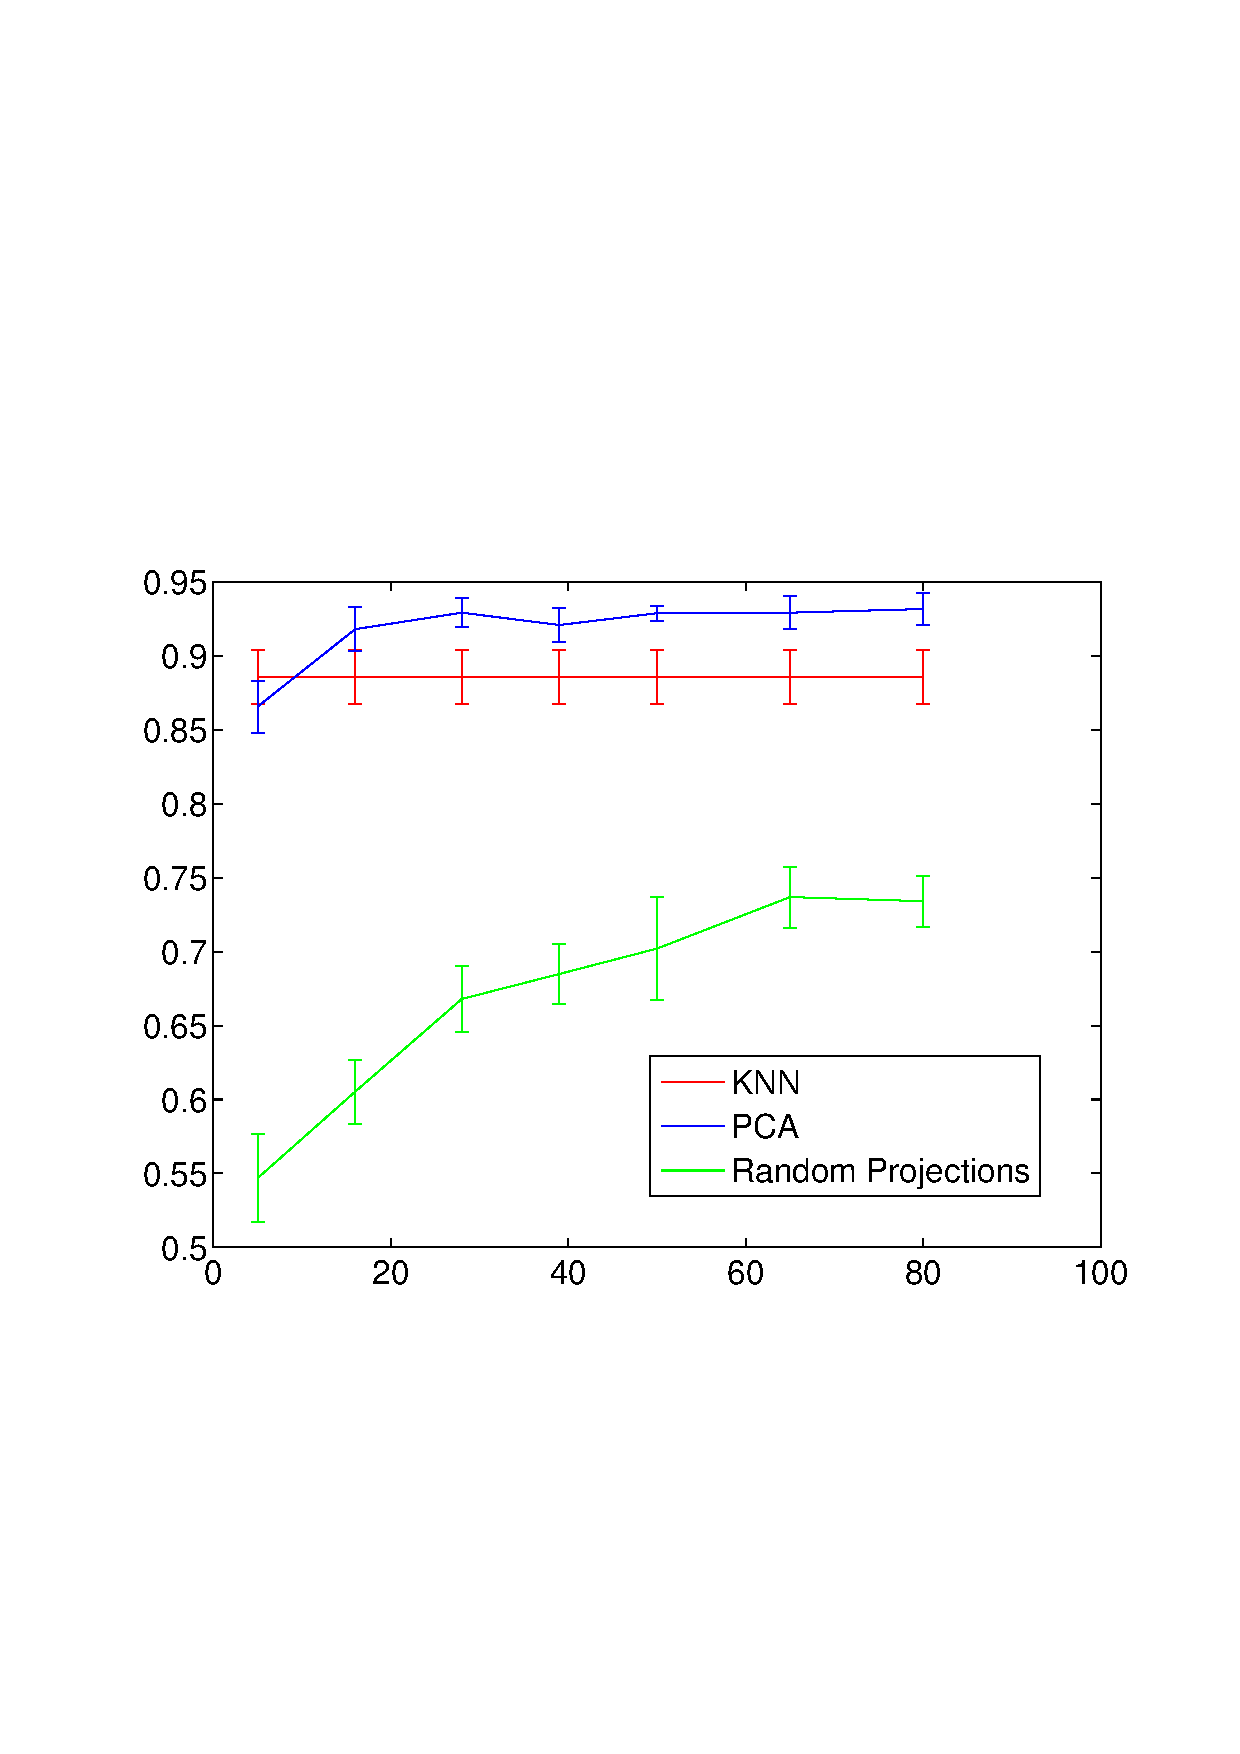
\includegraphics[width=.7\textwidth]{../images/knnVpcaVrproj.png}
\caption{Accuracy vs Dimensionality reduction size training with KNN.}
\label{fig:knn}
\end{figure}
\end{center}

